% --------------------------------------------------------------
% This is all preamble stuff that you don't have to worry about.
% Head down to where it says "Start here"
% --------------------------------------------------------------
 
\documentclass[12pt]{article}
 
\usepackage[margin=1in]{geometry} 
\usepackage{amsmath,amsthm,amssymb}
 
\newcommand{\N}{\mathbb{N}}
\newcommand{\Z}{\mathbb{Z}}
 
\newenvironment{intro}[2][I Introduction]{\begin{trivlist}
\item[\hskip \labelsep {\bfseries #1}\hskip \labelsep {\bfseries #2}]}{\end{trivlist}}

\newenvironment{p1}[2][II Dataset]{\begin{trivlist}
\item[\hskip \labelsep {\bfseries #1}\hskip \labelsep {\bfseries #2}]}{\end{trivlist}}

\newenvironment{p2}[2][III Feature Designs]{\begin{trivlist}
\item[\hskip \labelsep {\bfseries #1}\hskip \labelsep {\bfseries #2}]}{\end{trivlist}}

\newenvironment{p3}[2][IV Scoring Face Social Attributes with SVR]{\begin{trivlist}
\item[\hskip \labelsep {\bfseries #1}\hskip \labelsep {\bfseries #2}]}{\end{trivlist}}

\newenvironment{p4}[2][V Predicting Election Outcomes with Face Social Attributes]{\begin{trivlist}
\item[\hskip \labelsep {\bfseries #1}\hskip \labelsep {\bfseries #2}]}{\end{trivlist}}

\newenvironment{p5}[2][VI References]{\begin{trivlist}
\item[\hskip \labelsep {\bfseries #1}\hskip \labelsep {\bfseries #2}]}{\end{trivlist}}

\usepackage{graphicx}
\graphicspath{{./}}

\begin{document}
 
% --------------------------------------------------------------
%                         Start here
% --------------------------------------------------------------
 
\title{Project III Face Social Attributes and Political Elections Analysis by SVM}
\author{Yunzhong He\\ %replace with your name
204010749} %if necessary, replace with your course title
 
\maketitle

\begin{intro}{}
\item{}
For this project we studied the effects of face social attributes on political elections. In the first part we trained our classifier to face score social attributes such as "old", "rich", "masculine" etc. on novel faces, using ground truth information obtained from Amazon Turk workers[1]. In the second part we scored these social attributes on pairs of politicians who ran a electron against each other, and tried to predict the outcomes.
\end{intro}

\begin{p1}{}
\item{}
We used 491 500x500 jpg images that have scores for the 14 social attributes \{Old, Masculine, Baby-faced, Competent, Attractive, Energetic, Well-groomed, Intelligent, Honest, Generous, Trustworthy, Confident, Rich, Dominant\}, as training set to predict the scores of unseen photos. And we used 112 500x500 images of governor election candidates, 115 senator election candidates and their election outcomes as training set to predict election outcomes.
\end{p1}

\begin{p2}{}
\item{}
To be able to score social attributes on faces, we represent each image with a 1x119072 Histograms of Gradients (HoG) feature that indicates the images gradients at different regions. We also used a 160x1 vector to represent the positions of landmarks on a face. Below is an illustration of the features that we extracted from a governor's face.
\\
\begin{center}
		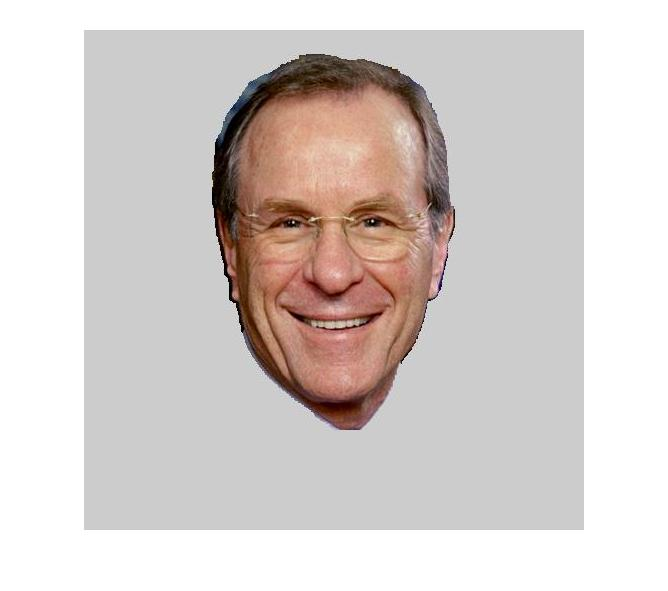
\includegraphics[height=4cm]{sample_feature_gov.jpg}
		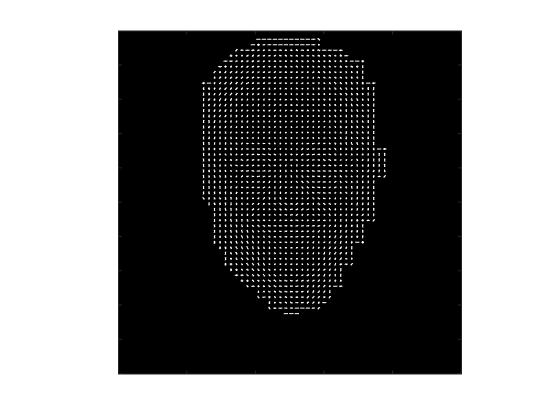
\includegraphics[height=4cm]{sample_feature_hog.jpg}
		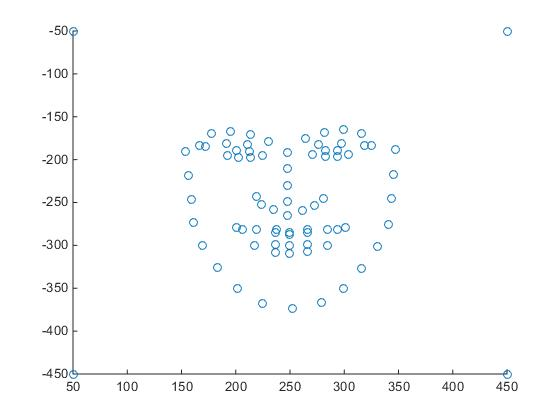
\includegraphics[height=4cm]{sample_feature_landmark.jpg}
		figure 1 governor, HoG feature and facial landmarks
\end{center}
The features are normalized into one long vectors. But since it is reasonable to believe that one entry in facial landmark is more informative than one entry in the HoG feature, we also optimized the weight of facial landmarks against HoG features for a best cross-validation accuracy.
\end{p2}

\begin{p3}{}
\item{}
To obtain scores of the 14 face social attributes we selected, we trained a SVR using the ground truth dataset for each face social attributes. And we obtained the following five fold cross-validation accuracy for each feature.\\
\begin{center}
	\begin{tabular}{||c c||} 
		\hline
	    Attributes  & Correlations\\
		\hline
		Old & 0.140923\\
		\hline
		Masculine & 0.093477\\
		\hline
		Baby-faced & 0.100584\\
		\hline
		Competent & 0.063177\\
		\hline
		Attractive & 0.100130\\
		\hline
		Energetic & 0.073559\\
		\hline
		Well-groomed & 0.069999\\
		\hline
		Intelligent & 0.051910\\
		\hline
		Honest & 0.052500\\
		\hline
		Generous & 0.050157\\
		\hline
		Trustworthy & 0.054232\\
		\hline
		Confident & 0.070558\\
		\hline
		Rich & 0.061880\\
		\hline
		Dominant & 0.070661\\
		\hline
	\end{tabular}
	{\\figure 2 regression errors}
\end{center}
And below is the regression reusult from one of the governor.\\
\begin{center}
		\includegraphics[height=7cm]{gov26_attributes.png}
		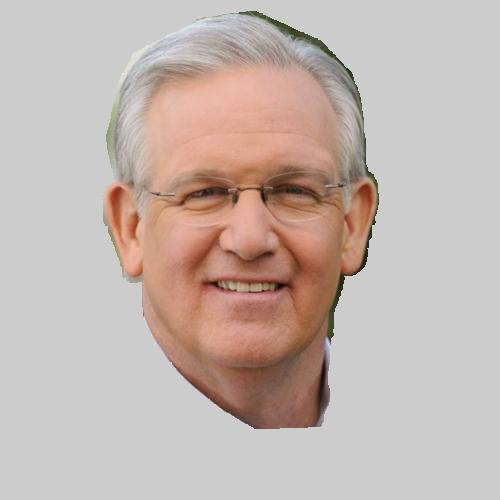
\includegraphics[height=7cm]{img-elec/governor/G0026.jpg}
		figure 3 face social attribute regression	
\end{center}
From figure 3 above we can tell that the governor candidate is old due to his grey hair, and his glasses may give people an impression of ingelligent. And it confirms with our regression results, in which old and intelligent had the largest values.
\item{}
\end{p3}

\begin{p4}{}
\item{V.1 Generate Training Data From Pairwise Election Results\\}
To generate positive and negative examples from pairwise election results, we splitted our datasets in half. And for the first half, we computed $f_{ab} = f_a - f_b$, where $f_a$ won over $f_b$, and we labeled them as positives. For the second half, we computed $f_{ba} = f_b - f_a$, where $f_a$ won over $f_b$, we labeled them as negative examples. So for governors we have 112/2 = 66 training examples, we for senators we have 116/2 = 68 examples.\\
\item{V.2 Predication Outcomes\\}
We trained a simple linear SVM based on the examples we computed from V.1, and performed 5-fold cross-validation. Below are the prediction accuracy we obtained.
\begin{center}
	\begin{tabular}{||c c||} 
		\hline
	    Campaign & Accuracy \\
		\hline
		Governor & 0.707\\
		Senator & 0.643\\
		\hline
	\end{tabular}
	{\\figure 4 predication accuracy}
\end{center}
From the figure 4 above we can see that the prediction outcomes are indeed better than random guesses, indicating that the election results is largely related to a candidate's look. And it also indicates that a the effect of facial apperance is more significant in a governor's campaign, this may or may not due to the fact that voters are generally more familiar with the candidates in senator campaigns than governor campaigns.\\
\item{}{V.3 Correlations\\}
We also computed the correlation of each face social attributes between the election outcomes, and below are the results.
\begin{center}
	\begin{tabular}{||c c||} 
		\hline
	    Attribute  & Mean squared error \\
		\hline
		Old & -0.162\\
		\hline
		Masculine & 0.167\\
		\hline
		Baby-faced & -0.06\\
		\hline
		Competent & -0.108\\
		\hline
		Attractive & 0.058\\
		\hline
		Energetic & 0.230\\
		\hline
		Well-groomed & 0.026\\
		\hline
		Intelligent & -0.008\\
		\hline
		Honest & -0.181\\
		\hline
		Generous & -0.166\\
		\hline
		Trustworthy & -0.119\\
		\hline
		Confident & 0.238\\
		\hline
		Rich & -0.006\\
		\hline
		Dominant & 0.262\\
		\hline
	\end{tabular}
	{\\figure 5 correlations}
\end{center}
Interestingly, we found that traits like 'dominant', 'confident', 'energetic' and even 'masculine' has the highest positive correlations between victory. This seems to suggest that people would prefer strong leaders. On the other hand, 'old' and 'generous', which may suggest a weak leader, have negative correlations. But traits like 'honest' and 'intelligent' also give negative correlations, which is very conterintuitive, and it may due to fact of having a relatively small sample size.
\end{p4}

\begin{p5}{}
\item{}
[1] J. Joo et al. "Automated Facial Trait Judgment and Election Outcome Prediction: Social Dimensions of Face," Int'l Conference on Computer Vision, 2015. 
\end{p5}

% --------------------------------------------------------------
%     You don't have to mess with anything below this line.
% --------------------------------------------------------------
 
\end{document}
